%!TEX program = xelatex
% 完整编译方法 1 pdflatex -> bibtex -> pdflatex -> pdflatex
% 完整编译方法 2: xelatex -> bibtex -> xelatex -> xelatex
\documentclass[lang=cn,11pt]{elegantpaper}

\title{A Bipartite Network Based Recommendation System via Network Embedding Augmented Collaborative Filtering Model }

\author{袁梦祥}
\institute{安徽大学大数据与云服务工程实验室}

% 不需要版本信息,直接注释即可
% \version{0.07}
% 不需要时间信息的话,需要把 \today 删除。
\date{}


% 参考文献样式 如果想修改参考文献样式,请把这行注释掉
%\usepackage[authoryear]{gbt7714}  % 国标

% 算法表格
\usepackage{algorithm}  
\usepackage{algpseudocode}  
\usepackage{amsmath}  
\renewcommand{\algorithmicrequire}{\textbf{Input:}}  
\renewcommand{\algorithmicensure}{\textbf{Output:}}

\begin{document}

\maketitle

\begin{abstract}
\noindent 使用推荐系统为用户提供个性化的推荐服务,有助于提高用户的满意度,更好的发掘物品的“长尾”。推荐算法是推荐系统的核心,基于协同过滤的推荐算法是目前应用比较广泛的推荐算法,但传统的协同过滤算法在推荐时存在数据稀疏量大,数据维数高,无法利用内容信息等问题。为了解决协同过滤算法的缺点,本文引入了网络表示学习的方法,使用二部图网络来表示用户的行为数据和项目的内容数据,再通过针对二部图结构设计的网络表示学习方法,学习网络中节点的低维度潜在表示,以获得用户和项目的领域信息。为了结合用户和项目的领域信息对用户进行推荐,我们进一步提出了一种融合领域信息的矩阵分解技术。本文结合协同过滤和嵌入算法的优点,提出了一种新的二部图推荐系统,该系统充分考虑了不同项目的内容特征和用户的行为偏好。我们在GoodBooks和Movielens数据集上对此方法进行了实验验证,结果表明,与其他推荐算法相比,基于网络表示学习的加强协同过滤算法有更好的推荐效果。
\keywords{推荐系统,二部图网络,网络表示学习,矩阵分解,协同过滤 }
\end{abstract}

% \lstinline{a4paper, 10pt} 自定义命令代表强调显示
% \begin{lstlisting}  \end{lstlisting} 自定义环境 代表一个代码块

\section{介绍}

在当今竞争激烈的市场环境下,产品的个性化程度已经成为影响顾客产品选择和满意度的重要因素。如果要给用户提供个性化的商品或服务,就必须充分研究用户的兴趣,而这正是推荐系统主要解决的问题,通过挖掘用户的历史行为数据,推荐系统可以自动发现用户的个性化需求。

推荐系统的本质是通过一定的方式将用户和项目联系起来,研究怎么将用户兴趣和项目关联起来的推荐算法是整个推荐系统的核心。早期的推荐方式是基于内容的推荐。基于内容的推荐算法[3] 也是常用的算法, 该算法通过整理用户过去喜欢的物品信息, 找出与之相似度高的
物品对目标用户进行推荐。该算法在计算物品相似度
的基础上分析用户和物品的内部信息, 通过用户的喜好
和物品的属性来进行推荐。该算法在考虑用户喜好的
同时也达到了推荐结果直观且便于理解的作用。但是
该算法处理非文本信息难度比较高, 比如音乐、图像等

目前应用最广泛的推荐算法是协同过滤类别的推荐算法,因此也有许多关于该算法的研究\cite{Linden2003},该算法的核心是相似度计算,Badrul Sarwar等在论文里做了详细的研究\cite{Sarwar2001}。传统的相似度计算依赖用户的行为,然而在实际应用中,用户的行为受流行度影响较大,用户的行为矩阵通常比较稀疏,这导致相似度的计算结果不稳定。

基于模型(model based)的协同过滤是目前最主流的协同过滤类型了,我们的一大堆机器学习算法也可以在这里找到用武之地。机器学习时代矩阵分解算法


深度学习的来临,矩阵分解算法只能学习到用户和物品的线性关系,


与现有的工作不同,本文使用网络表示学习的方法,将项目和用户映射到低维向量空间。使用二部图网络来表示数据,,最后该系统集成了矩阵分解模型,一个好的推荐系统不仅能给用户提供推荐,也能反应出用户喜欢的程度,结合矩阵分解模型,可以给用户的产生基于评分的推荐,同时解决i系统的冷启动问题\cite{Qiu2011}。


总之,本文的主要贡献有三方面:
\begin{itemize}
	\item 本论文采取表示学习的方式,学习到用户和行为的低维度向量表示,再结合矩阵分解和协同过滤的方法,实现评分预测和用户个性化推荐。
	
	\item 使用二部图表示用户的行为数据和物品的内容信息。然后,通过网络表示学习的算法,将用户根据行为数据,物品根据内容信息分别映射到不同的嵌入向量空间。最后在嵌入向量空间中比较用户之间和物品之间的相似度,利用协同过滤的思想对原始评分矩阵进行填充。
	
	\item 不仅能给用户提供推荐,也能反应出喜欢的程度。
\end{itemize}

本文的其余部分安排如下。第二节介绍了相关的工作; 第三节详细介绍了推荐模型的整体架构; 第四节介绍了实验; 最后,第五节总结论文并讨论论文的未来工作。


\section{相关工作}

我们的工作涉及到协同过滤、基于二部图网络的推荐和基于网络表示学习的二部图。因此,在本节中,我们将简要回顾这些领域的相关工作。

\subsection{协同过滤}
基于用户的历史交互行为,对用户产生推荐的方法主要是基于协同过滤(CF)思想的\cite{Su2009},其目的是用静态的潜在特征向量表示用户和条目。矩阵分解(MF)是实现协同过滤最常用的方法。基本的MF模型,如[13,14]尝试学习用户和项目的潜在功能完全通过匹配用户-项目的交互(即。,二进制指标或用户-项目评分)矩阵与点积(DP)操作。然后,通过对给定的用户-项目对使用派生的用户/项目潜在特性的DP操作,计算评级预测。大量的工作试图通过基于用户-项目交互的建模来提高MF的性能。例如,[14]在MF中引入了用户和项目偏差。[15]将邻域建模集成到MF中。它假定用户对某一项的评价不仅由用户对该项的潜在特征构成,而且还由用户对其他项的评价行为构成。这些方法在许多领域的性能都优于传统的MF模型。然而,所有这些基于MF的模型都使用DP操作作为其评级预测器。DP操作的一个固有限制是潜在特征相互独立。也就是说,DP只支持潜在特征的线性组合,而不考虑高阶特征交互。实验结果表明,现有的基于MF的方法性能较差。

\subsection{网络表示学习}

二部网络是一种普遍存在的数据结构,用于对两类实体之间的关系进行建模。它在推荐系统、搜索引擎、问答系统等方面得到了广泛的应用。例如,在搜索引擎中,查询和网页形成一个二部图网络,边缘可以指示用户点击行为,提供有价值的关联信号[1,2];在推荐系统的另一个应用中,用户和项目形成一个二部网络,边缘可以编码包含丰富的协同过滤模式[3]的用户评价行为。要对网络数据执行预测分析,首先获得表示形式(即,特征向量)表示顶点。传统的向量空间方法,如袋装词表示方法,在处理大规模动态网络的实际应用中,语义捕获太少,效率低下。近年来,数据挖掘和信息检索领域的研究主要集中在从数据中学习表示[4 7]。特别是,它们将顶点嵌入到低维空间中,即,将顶点表示为可学习的嵌入向量。基于顶点嵌入的标准机器学习技术可以应用于各种预测任务,如顶点标记、链接预测、聚类等。




\section{推荐模型}

使用图嵌入的方式,将用户-物品的二部图表示转化为低维度的向量,在低维度向量空间中,考虑相似性,最后结合矩阵分解和协同过滤模型,通过机器学习的方式填充评分矩阵,完成个性化推荐。

融合领域信息的矩阵分解的loss函数如下:


\subsection{算法}

这里介绍模型使用的算法

\begin{algorithm}[h]  
	\caption{Conjugate Gradient Algorithm with Dynamic Step-Size Control}  
	\label{alg::conjugateGradient}  
	\begin{algorithmic}[1]  
		\Require  
		$f(x)$: objective funtion;  
		$x_0$: initial solution;  
		$s$: step size;  
		\Ensure  
		optimal $x^{*}$  
		\State initial $g_0=0$ and $d_0=0$;  
		\Repeat  
		\State compute gradient directions $g_k=\bigtriangledown f(x_k)$;  
		\State compute Polak-Ribiere parameter $\beta_k=\frac{g_k^{T}(g_k-g_{k-1})}{\parallel g_{k-1} \parallel^{2}}$;  
		\State compute the conjugate directions $d_k=-g_k+\beta_k d_{k-1}$;  
		\State compute the step size $\alpha_k=s/\parallel d_k \parallel_{2}$;  
		\Until{($f(x_k)>f(x_{k-1})$)}  
	\end{algorithmic}  
\end{algorithm}  




\subsection{算法模型图}

介绍算法的模型

\begin{figure}[h]
	\centering
	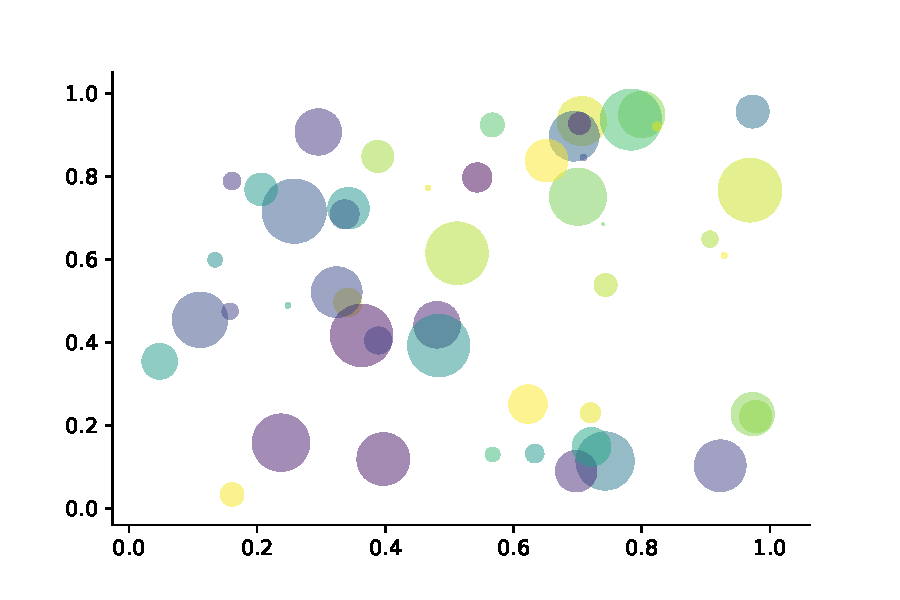
\includegraphics[width=0.6\textwidth]{imgs/scatter.pdf}
	\caption{Scatter Plot Example \label{fig:scatter}}
\end{figure}


\section{实验}
实验部分,介绍论文的实验

我强烈建议你使用 \lstinline{booktabs} 宏包,这个宏包有三个命令 \lstinline{\toprule}、\lstinline{\midrule} 和 \lstinline{\bottomrule} 能方便你制作三线表。图\ref{fig:scatter} 是一个示例:



\section{结论和未来工作}
结论部分,介绍论文的实验结果

\nocite{*} 代表显示所有的论文文献 包括文中没有引用的

% 如果想修改参考文献样式(非国标),请把下行取消注释,并换成合适的样式(比如 unsrt,plain 样式)。
\bibliographystyle{unsrt}
\bibliography{wpref}

\end{document}
